\chapter{Matter and Energy}

The universe is made of matter and energy. Current models posit that the universe
is approximately 68\% dark energy, 27\% dark matter, and 5\% ordinary matter. 
Everything you can see and touch is part of the small part of the universe made 
of ordinary matter. Most science deals with ordinary matter and its interactions; 
highly trained theoretical physicists are currently debating the nature and 
effects of dark matter and dark energy. 
\begin{wrapfigure}{r}{2.5in}
\noindent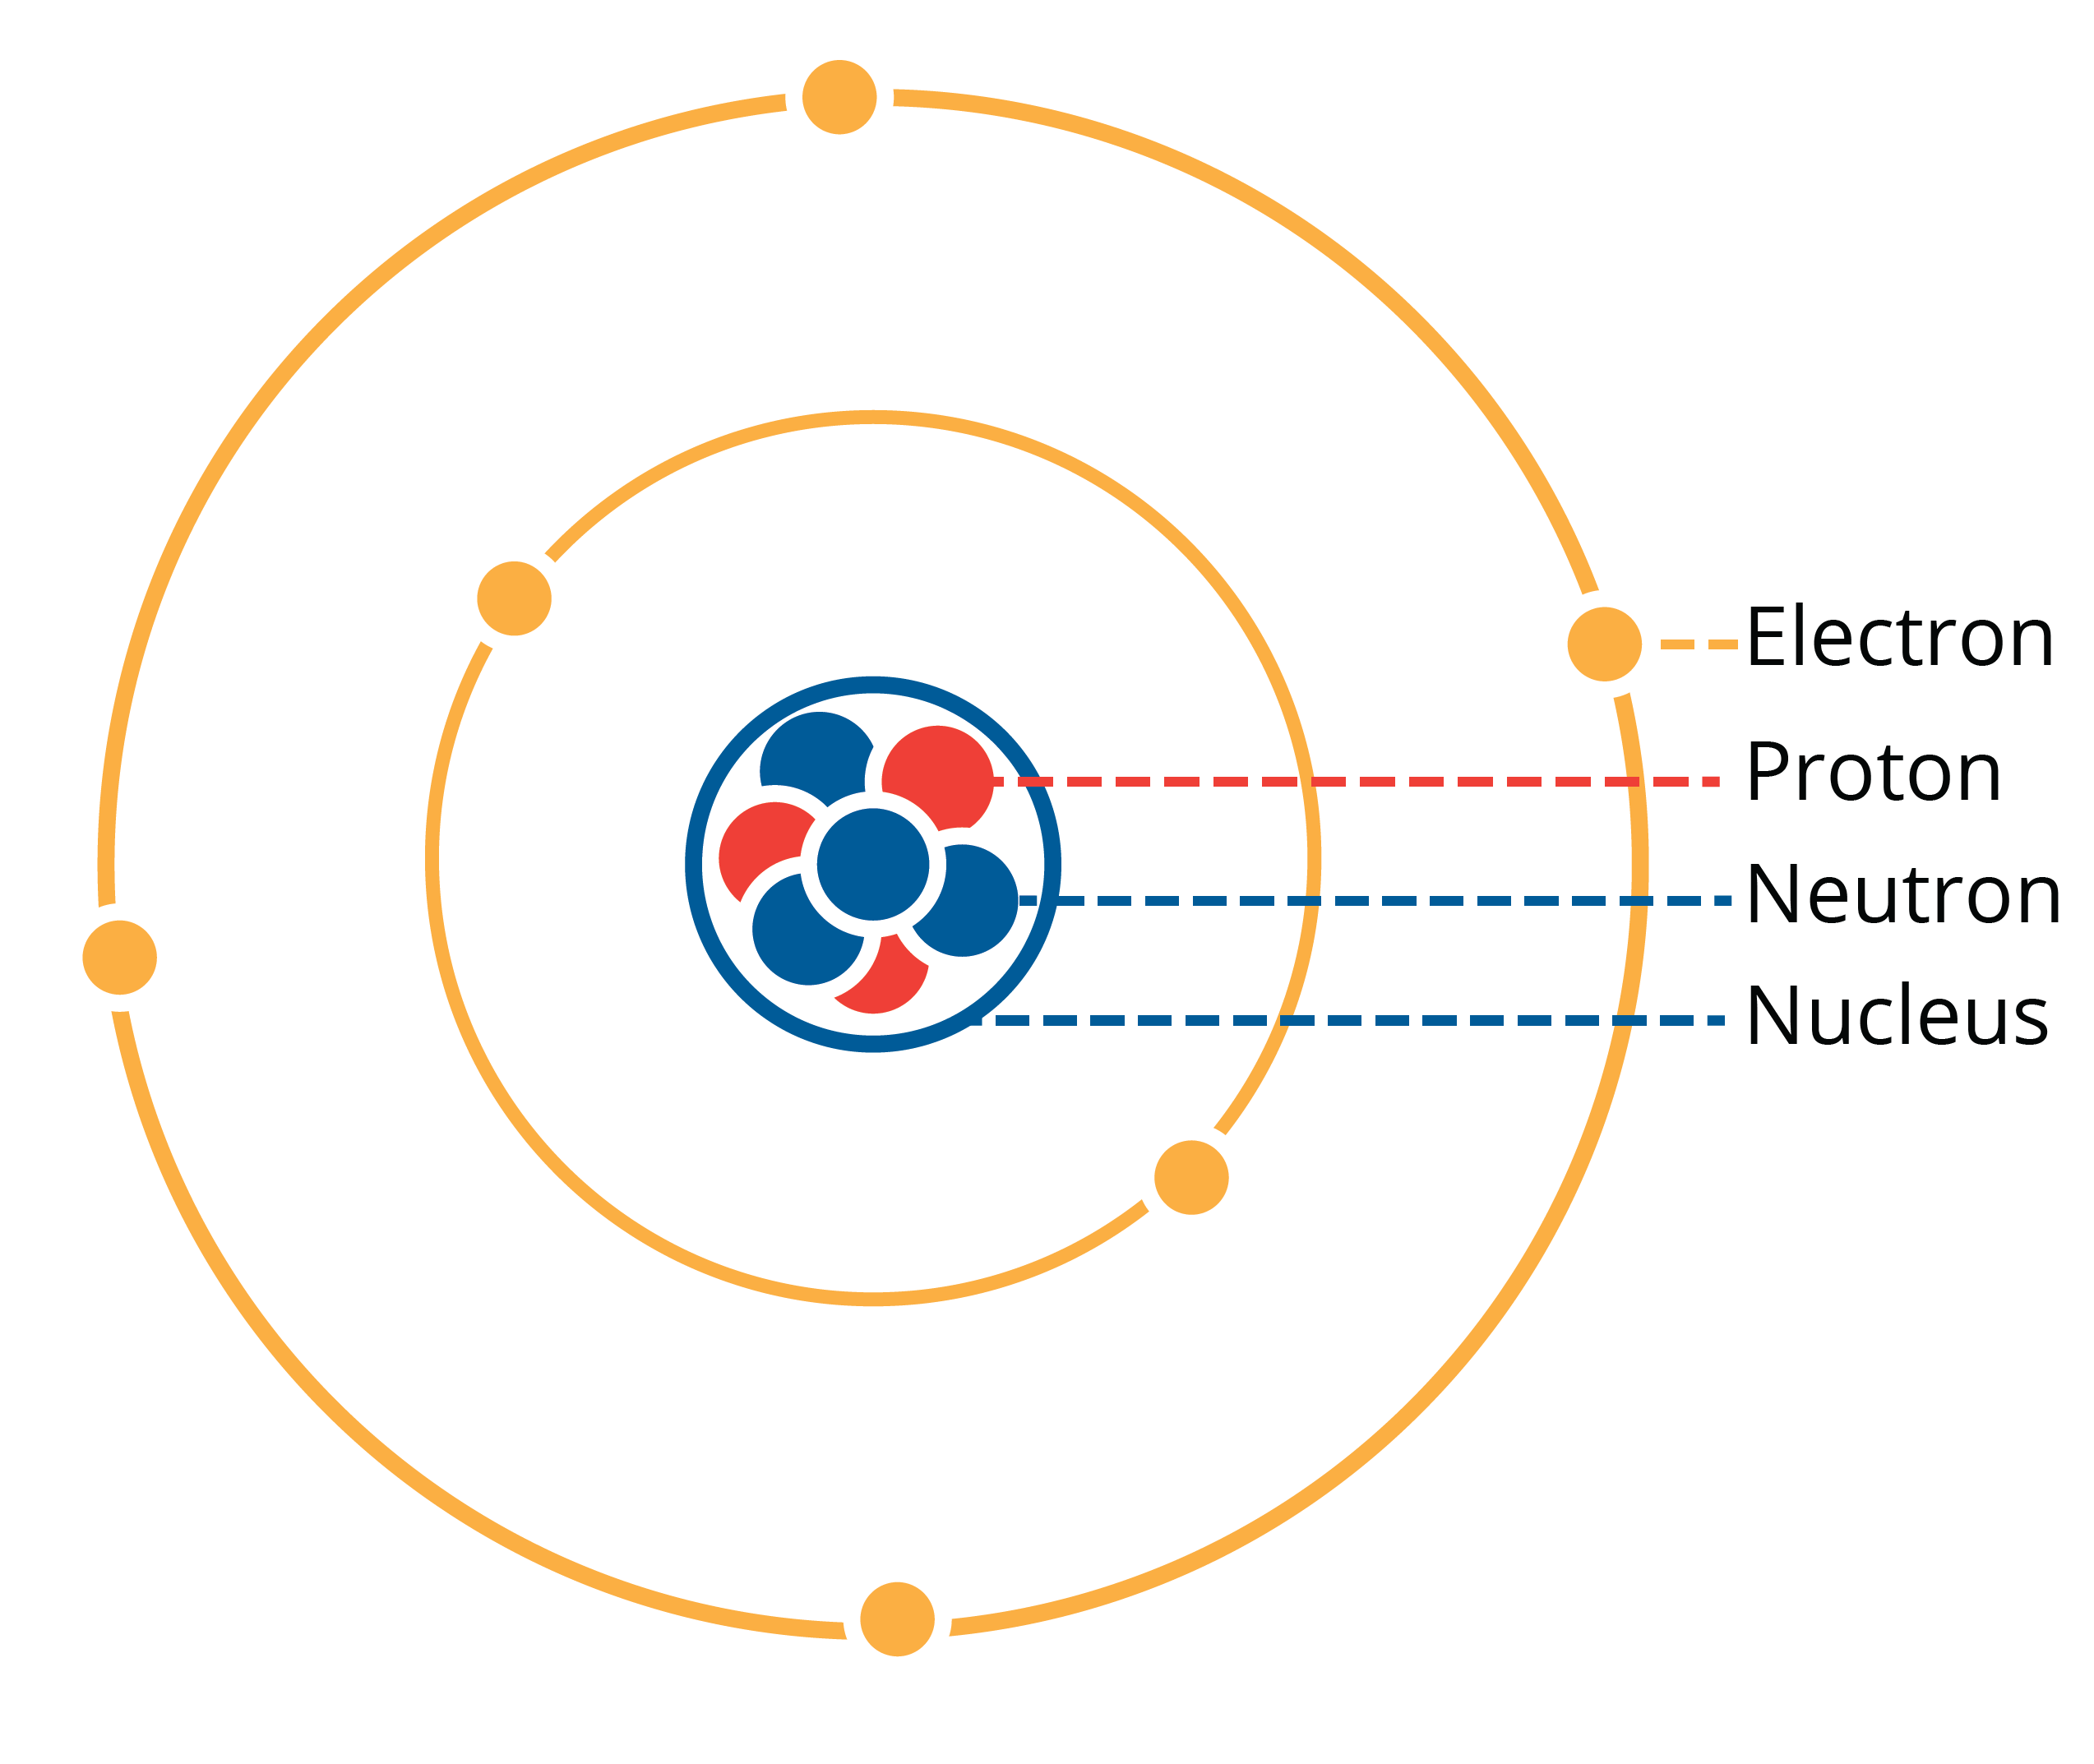
\includegraphics[width=2.5in]{atom1.png}
\caption{}
\label{fig:atom1}
\end{wrapfigure}

What is this ordinary matter made of? All things (including the air around you) 
are made of atoms. Atoms are incredibly tiny --- there are more atoms in a drop 
of water than there are drops of water in all the oceans.
% ADD: If you want a better visual of the scale: https://htwins.net/scale2/, start at around 10^-8

Every atom has a nucleus that contains protons and neutrons. Orbiting around the
nucleus is a cloud of electrons. However, the mass of the atom comes mainly from 
the protons and neutrons, since they are about 2000 times as massive as an 
electron! These three particles, protons, neutrons, and electrons, are called
\textit{subatomic particles}. (See figure \ref{fig:atom1}.) \index{protons} 
\index{neutrons} \index{electrons} \index{subatomic particle}

\section{Atoms and Their Models}
Over the history of science, there have been many ideas about the structure of
atoms. This history is a good example of how science develops: unexpected
results drive scientists to update their models, moving us closer and closer to
a true model of the atom.

During his investigations into the behavior of gases, John Dalton noted that 
different elements combine in strict ratios. For example, he noted that nitrogen 
and oxygen combine in a 1:1 and 1:2 fashion, but no ratio in between.

\begin{wrapfigure}{l}{3in}
\noindent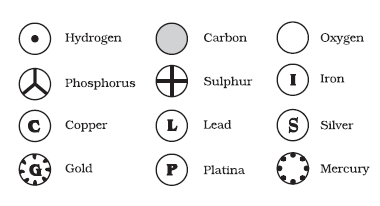
\includegraphics[width=2.5in, trim={0 0.5cm 0 0.5cm}, clip=true]{daltons_model.png}
\caption{Dalton modeled atoms as indivisible and unique.}
\end{wrapfigure}

This first model of the atom is rudimentary; each element is a unique atom,
and those atoms cannot be subdivided. The atom is modeled as one large, solid,
uniform, and neutral object. British physicist J.J. Thomson discovered that
atoms could be split into a light, negatively charged particle and a heavier,
positively charged particle (we now know this is the nucleus, the dense
grouping of protons and neutrons in the center of an atom).

Suddenly, the atom went from neutral and indivisible to made of different types
of charged particles. Further experiments by Ernest Rutherford showed the atom
to be mainly empty space, further updating scientists' model of the atom.
Subsequently, Bohr explained the phenomena of spectral lines (we will discuss
this further in Sequence 2) by modeling electrons as being restricted to
orbiting specific distances from the nucleus.

\begin{wrapfigure}{r}{3in}
\noindent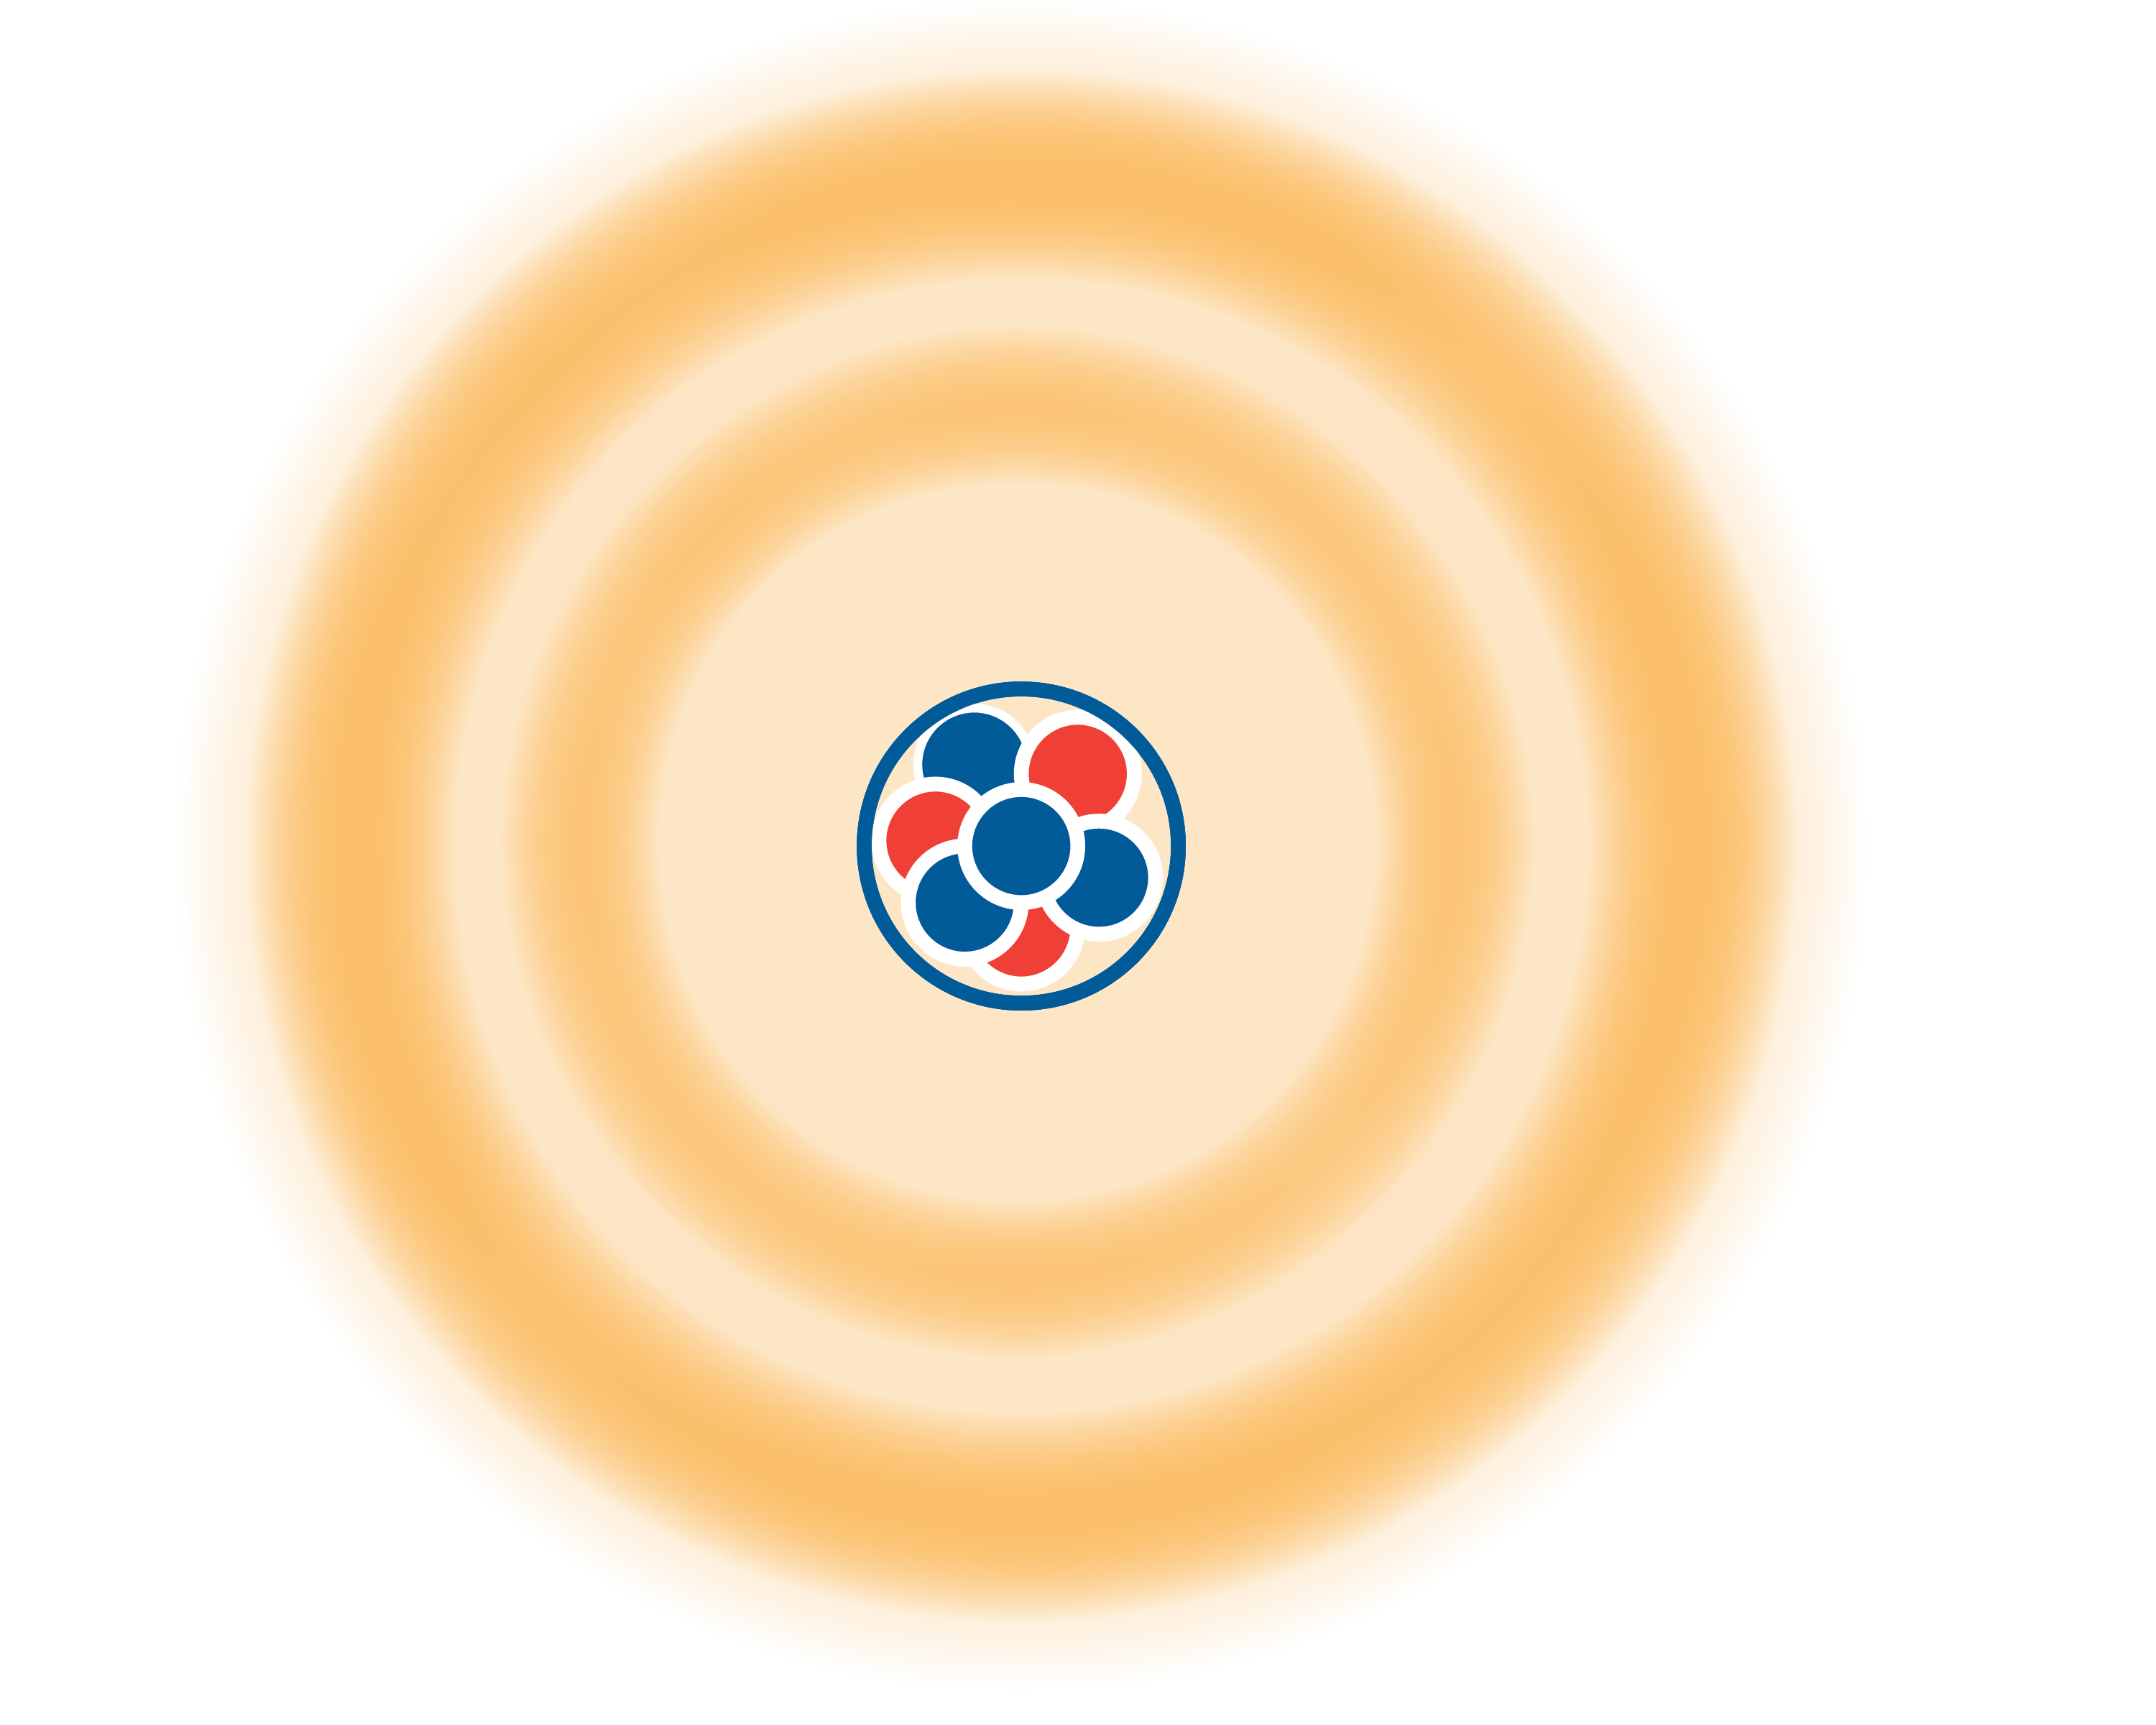
\includegraphics[width=3in]{atomCloud.png}
\caption{}
\label{fig:atomCloud}
\end{wrapfigure}

This is likely the model you are most familiar with seeing, and it is the one we
will use most often in this text. The first figure shown in this chapter is a Bohr
model: it shows the protons and neutrons in the nucleus, and models the electrons 
as moving in discrete orbits around the nucleus. 

However, the Bohr model is slightly inaccurate. While it is a convenient model for
thinking about atoms, in reality, electrons don't neatly orbit the nucleus.
Scientists don't know exactly where an electron will be in relation to the
nucleus, but they do know where it is most likely to be. They use a cloud that is
thicker in the center but fades out at the edges to represent an electron's
position (see figure \ref{fig:atomCloud}).

\begin{wrapfigure}{r}{3in}
\noindent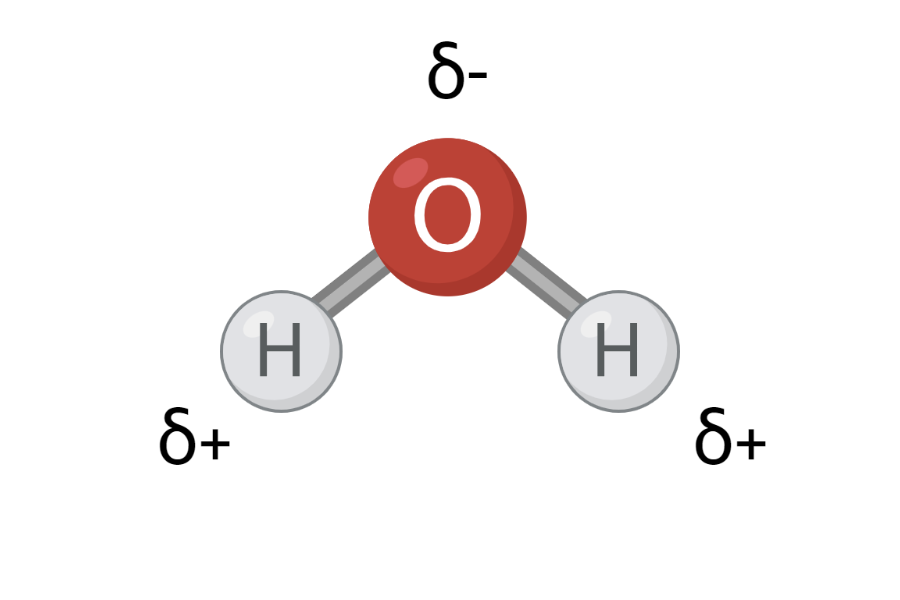
\includegraphics[width=3in]{water_polar.png}
\caption{}
\label{fig:water_polar}
\end{wrapfigure}

While the cloud model is more accurate, we will use the Bohr model as it
allows the viewer to easily and quickly assess the number and arrangement of
electrons.

\subsection{Classifying Atoms}

We classify atoms by the numbers of protons they have. An atom with one proton
is a hydrogen atom, an atom with two protons is a helium atom, and so forth
(refer to periodic table on pg..). We say that hydrogen and helium are \textit{
elements} because the classification of elements is based on the proton number.
And we give each element an atomic symbol. Hydrogen gets $H$, helium gets $He$,
oxygen gets $O$, carbon gets $C$\index{elements}, and so on.

\subsection{When Atoms Combine}
When atoms of different elements combine, they make \textit{compounds}. Compounds
are substances made up of more than one element. Compounds can be 
\textit{molecules} or \textit{crystal lattices}. In the next section you'll learn
\textit{why} these different structures form. 

There are many kinds of compounds. You know a few:
\begin{itemize}
\item Table salt is crystals made of $Na^{+}$ and $Cl^{-}$ ions: a sodium atom 
that as lost an electron and a chlorine atom that gained an electron
\item Baking soda, or sodium bicarbonate, is $NaHCO_3$.
\item $O_2$ is the oxygen molecules that you breathe out of the air (air, a
blend of gases, is mostly $N_2$.).
\item Common quartz is $SiO_2$: silicon dioxide
\end{itemize}

The subscripts indicate what ratio of the elements are present in the compound. 
Each number indicates the ratio for the preceding element. A drop of water, 
$H_2O$, has twice as many hydrogen atoms as oxygen atoms. 

\textbf{Example}: What is the ratio of elements present in Epsom salt?

\textbf{Solution}: Epsom salt, chemical name magnesium sulfate, has the chemical formula $MgSO_4$. Therefore, the ratio of Mg:S:O is 1:1:4. 

%fixme molecule vs formula unit, ordering of bonds versus formulas

\begin{Exercise}[title = {Numbers of Atoms in Molecules}, label = num_atom]
Give the elemental ratio for each compound. 
\begin{enumerate}
\item methane, $CH_4$
\item copper (II) sulfate, $CuSO_4$
\item glucose, $C_6H_{12}O_6$
\end{enumerate}
\end{Exercise}

\begin{Answer}[ref = num_atom]
\begin{enumerate}
\item C:H = 1:4
\item Cu:S:O = 1:1:4
\item C:H:O = 6:12:6 = 1:2:1
\end{enumerate}
\end{Answer}

\section{Types of Matter}
One way to classify matter is by the types of chemical bonds that hold a 
material's atoms together. The nature of these bonds, in turn, affects the 
properties of the material. For now, all you need to know is there are three types
of chemical bonds: metallic, covalent, and ionic. Materials held together with the
same type of bonds tend to have similar properties. For example, copper, bronze, 
iron, and steel (all containing metallic bonds) are all shiny, ductile, malleable,
and good conductors of heat and electricity. On the other hand, Epsom salt and 
table salt for large crystals, have very high melting points, and are poor 
conductors of electricity in their pure form. These two substances (Epsom and 
table salt) both contain ionic bonds. 

\subsection{Ionic Compounds}
Ionic bonds are the electrical attraction between opposite-charged ions. When a 
neutral atom gains or loses an electron it becomes an \textit{ion} (a charged 
atom), and oppositely-charged ions are attracted to each other. Which atom gets 
the electron and which loses it is based on their relative 
\textit{electronegativities}.\index{electronegativity} Electronegativity is simply
a measure of how strongly an atom can attract electrons to itself. In general, 
elements on the right side of the periodic table are more electronegative than 
elements on the left side. There are also polyatomic ions: groups of atoms held 
together with covalent bonds that have an overall charge (figure ... shows a Bohr 
model of a phosphate polyatomic ion, as an example). For now, we'll focus just on 
ionic bonds between monoatomic ions, like in table salt. You'll learn more about 
polyatomic ions and the compounds they form in Sequence 2. 

\begin{wrapfigure}{l}{3in}
\noindent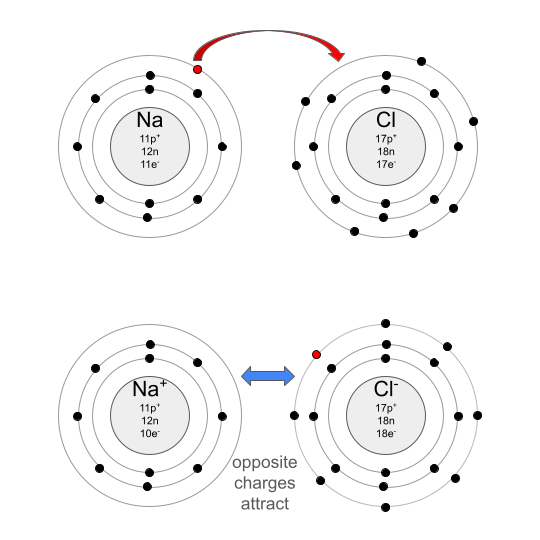
\includegraphics[width=3in]{NaCl_xfer.png}
\caption{}
\label{fig:NaCl_xfer}
\end{wrapfigure}

Let's examine how a simple ionic compound is formed: sodium chloride, also known 
as table salt, is made up of sodium and chlorine atoms (see figure 
\ref{fig:NaCl_xfer}). When sodium and chlorine come in contact with each other, 
electrons move from the sodium to the chlorine, making a sodium \textit{cation} 
(positively-charged ion) and a chloride \textit{anion} (negatively-charged ion). 
Yes --- chlor\textit{ide} is correct! When naming an anion, the ending of the 
element name changes to \textit{-ide}. Once the sodium cation and chloride anion 
are formed, their opposite charges attract them to each other, like north and 
south magnet poles. 

\begin{wrapfigure}{l}{3in}
\noindent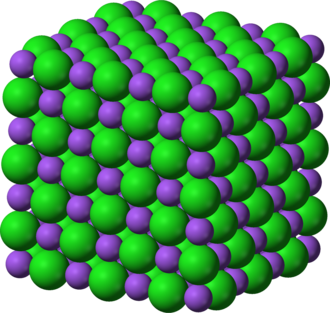
\includegraphics[width=2in]{NaCl_lattice.png}
\caption{}
\label{fig:NaCl_lattice}
\end{wrapfigure}

When there are many, many sodium and chloride ions around, they spontaneously 
arrange themselves in a pattern, giving ionic compounds their characteristic 
crystal structure (see figure \ref{fig:NaCl_lattice}). Because the electrons are 
tightly held be each ion, ionic substances don't conduct electricity well as 
solids. The atomic crystal lattice also determines the shape of the macroscopic 
crystals. Salt crystals are generally cubic, while other crystals (like quartz) 
form hexagonal prisms. You'll learn how to predict the atomic and macroscopic 
crystal structure of different compounds in Sequence 2. 

\subsection{Covalent Compounds}
Water is an example of a covalent compound: it is made of two hydrogen atoms 
covalently bonded one oxygen atom (see figure \ref{fig:water_polar}). The result 
is a water molecule\index{molecules}. The different atoms cluster together 
because they share electrons in their clouds. This is the nature of a 
\textit{covalent bond}\index{covalent bond}: it is formed when atoms share electrons.
Sometimes, electrons are shared evenly, but in water, they are shared unevenly. 
Due to the difference in electronegativity between hydrogen and oxygen, the 
shared electrons are more attracted to the oxygen atom than the hydrogen atoms, 
so they spend more time on the oxygen atom. As a result, the oxygen side of a 
water molecule has a slight negative charge, while the hydrogen atoms have a 
slight positive charge. The slight charges are represented with a lower case 
Greek letter delta, $\delta$. When electrons are shared unevenly, we call this a
\textit{polar} covalent bond, because there are positive and negative poles at 
either end of the bond. \index{polar bond} \index{non-polar bond}

When covalent bonds form between two elements of similar electronegativities, 
the electrons are shared evenly. We call this a \textit{non-polar} covalent bond. 
Oil is an example of a non-polar covalent substance. Different oils have different
combinations, but all oils are made mainly of carbon and hydrogen, which have similar
electronegativities. For both polar and non-polar covalent bonds, the electrons 
are still held tightly, even if they are shared. Those electrons don't move to 
another molecule: they move around within the molecule they are already a part 
of. Since electrons don't flow freely in covalent substances, they are also poor 
conductors of electricity. But, they generally have lower melting and boiling 
points than ionic compounds. 

What happens when you try to mix oil and water? They don't mix well! This is due 
to the difference between their bond types. Polar substances, like water, mix best
with other polar substances, while non-polar substances, like oils, mix best with 
non-polar substances. You'll learn more about why this is in Sequence 2.

\subsection{Metallic Compounds}
You may already know that metals (both pure and alloyed) are excellent conductors of electricity and heat. This is a consequence of their metallic bonds. 
%fixme complete section, pure vs alloys, free flowing electrons



\section{Energy and Work}

Energy is defined as the ability to do work, but what does this mean? First, we 
need to understand what \textit{work} is. When you lift an object into the air, 
you are doing work on that object. When water turns a turbine in a hydroelectric 
plant, the water is doing work on the turbine. And when you hit the brakes on your
car, the brake pads are doing work on the tires (albeit, negative work). 
\textit{Energy} is being transferred between these pairs of objects when work is 
done. 

Some everyday examples of energy include:
\begin{enumerate}
\item The Calories in your food
\item The light from the Sun
\item Heat in the Earth's mantle
\item The motion of a spinning wheel
\end{enumerate}

Some types of energy are easy to visualize, while others are not. Energy is what 
moves from one object to another when work is being done. When you lift 
something, the energy stored in your body (in the form of sugar and fat) is 
transferred to the object, accelerating it upwards. Your body continues to 
transfer energy as you lift the object against gravity. When you've lifted it as 
high as you can, most of the energy your body lost (we call this "burning 
Calories" colloquially) is stored as \textit{potential energy}, due to the 
object's height. 

Another example is a simple circuit connecting a battery and a light bulb. The 
battery has stored potential energy. When the circuit is complete, the potential 
energy in the battery is transferred to electrons in the light bulb, causing them 
to move and gain kinetic energy. In the light bulb's filament (we are referencing 
old, non-LED light bulbs here!), the electrons encounter resistance, which slows 
them down. The energy the electrons lose in this process is being transformed into 
light and heat, lighting your room. 

%fixme edit/rehome material below



\section{Chemical Reactions}

\begin{wrapfigure}{l}{3in}
\noindent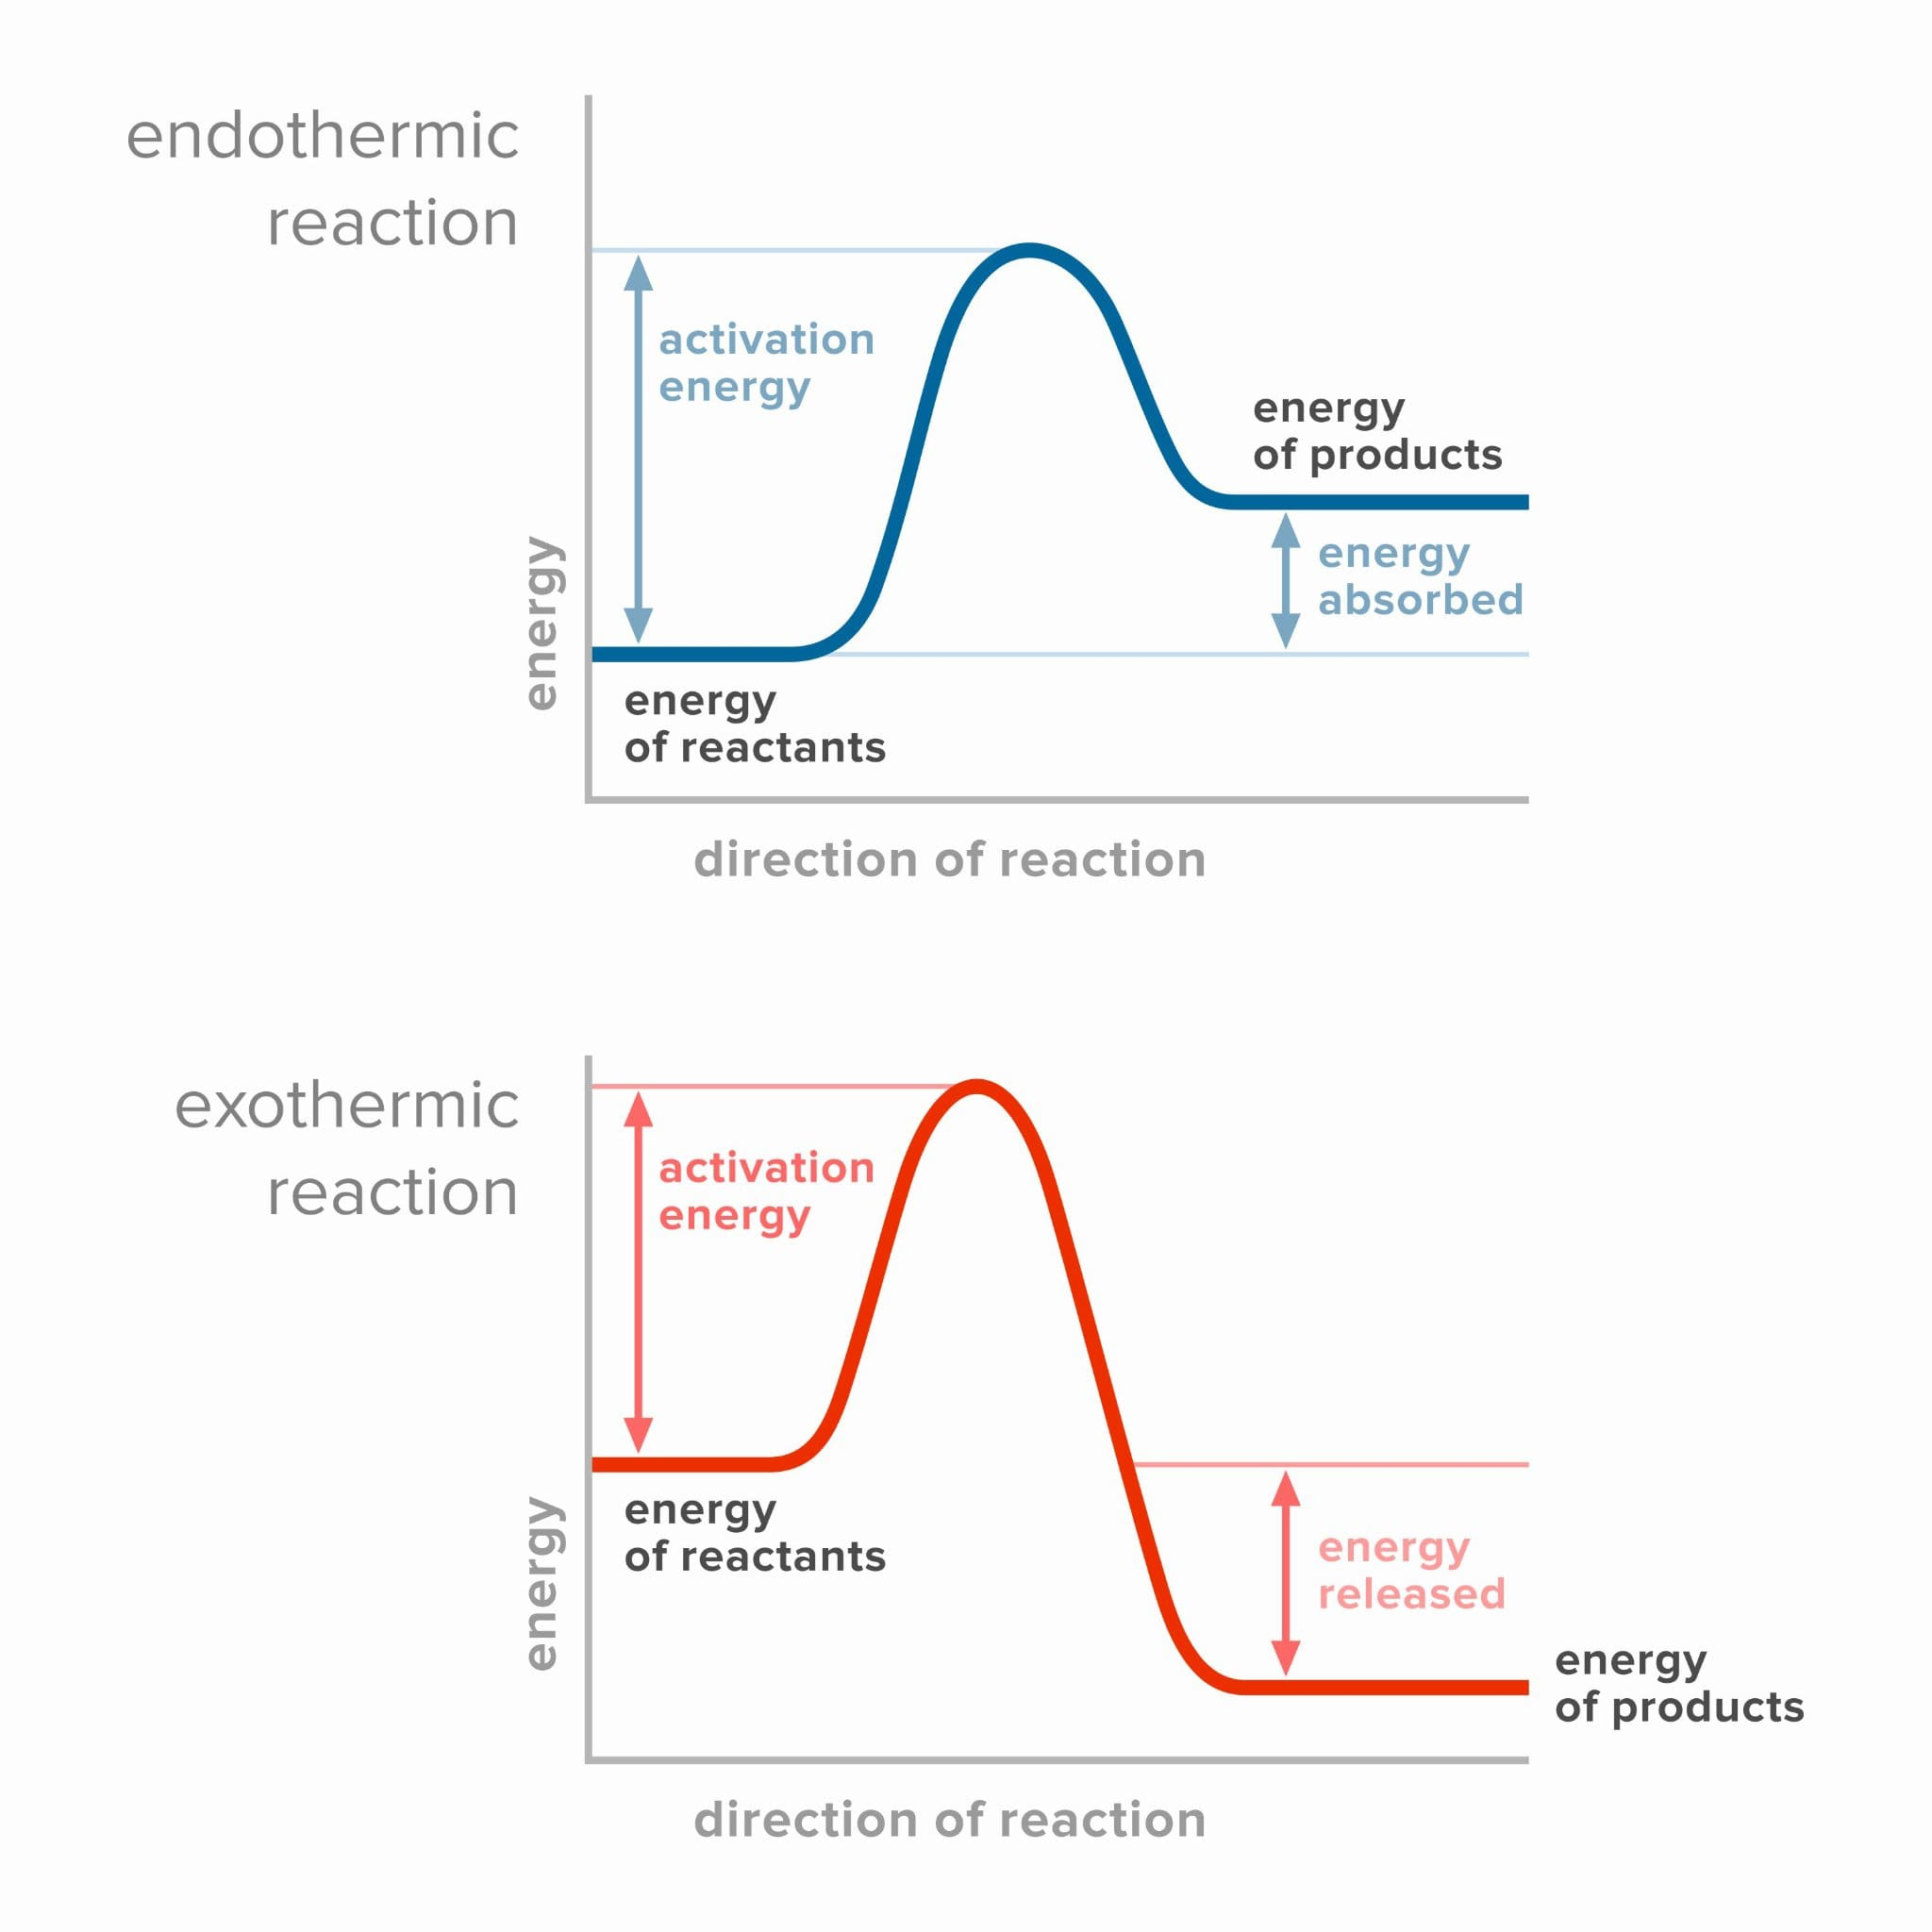
\includegraphics[width=3in]{exo_endo_diagrams.png}
\caption{}
\label{fig:exo_endo_diagrams}
\end{wrapfigure}

Sometimes two hydrogen atoms form a molecule ($H_2$). Sometimes two oxygen
atoms form a molecule ($O_2$). If you mix these together and light a match,
they will rearrange themselves into water molecules. This is called a \textit{
chemical reaction}. In any chemical reaction, the atoms are rearranged into new
molecules.\index{chemical reaction}

Some chemical reactions (like the burning of hydrogen gas described above) are
\textit{exothermic} --- that is, they give off energy. Burning hydrogen gas
happens quickly and gives off a lot of energy. If you have enough, it will make
quite an explosion! \index{exothermic}

Other chemical reactions are \textit{endothermic} --- they consume energy.
Photosynthesis, the process by which plants consume energy from the sun to make
sugar from $CO_2$ and $H_2O$ requires an endothermic chemical reaction.\index{endothermic}

Examine the diagrams in figure \ref{fig:exo_endo_diagrams}. The $x$-axis 
represents time - time passes as wemove from left to right across the diagram. 
At the far left, the energy of the reactants (the ingredients that go into the 
reaction) is shown. At the far right, the energy of the products (what is made in 
the chemical reaction) is shown. The red diagrams shows an exothermic reaction: 
the products (what is made) have less energy than the reactants (the "ingredients"
that start the reaction). Since energy is never created or destroyed, where did 
the energy go? It is released as heat. So, exothermic reactions release heat.

Now, look at the endothermic reaction diagram (the blue one). Based on the
relative energies of the reactants and products, do you expect and endothermic
reaction to release or absorb heat? Absorb! Since the products have more
energy, they must have absorbed energy, in the form of heat, from the surroundings.

What does this look and feel like in real life? If an exothermic reaction were
happening in a glass beaker, you would feel warmth if you held the beaker. The
heat is leaving the beaker and entering your hand, which feels warm. What
about an endothermic reaction? Many students think that since an endothermic
reaction absorbs heat, it must be getting hot. This is incorrect:
\textit{exothermic} reactions feel hot. If an endothermic reaction were
happening in a beaker and you touched the beaker, it would feel \textbf{cold}.
Why? Well, if the reaction is absorbing heat, then heat must be leaving it
surroundings (your hand) and entering the reaction (this heat energy is turned
into chemical energy that is stored in the new chemical bonds that are
forming). So your hand feels cold. %fixme: models showing flow of heat in/out of system for chemical reactions.

\section{Mass and Acceleration}

Each atom has a mass, which means everything made up of those atoms has mass as 
well (and that's pretty much everything!). We measure mass in grams. A paper clip 
is about 1 gram of steel. An adult human can have a mass of 70,000 grams, so for 
larger things, we often talk about kilograms, which is 1000 grams.

The first interesting thing about mass is that objects with more mass
require more force to accelerate. For example, pushing a bicycle so
that it accelerates from a standstill to jogging speed in 2 seconds
requires much less force than pushing a train so that it accelerates
at the same rate.


\begin{mdframed}[style=important, frametitle={Newton's Second Law of Motion}]

The force necessary to accelerate an object of mass $m$ at an acceleration of
$a$ is given by:
$$F = m a$$

This means the force is equal to the mass times the acceleration.

\end{mdframed}

What are the units here? We already know that mass is measured in
kilograms. We can measure velocity in meters per second, but that is
different from acceleration. Acceleration is the rate of change in
velocity. So if we want to go from 0 to 5 meters per second (that's
jogging speed) in two seconds, that is a change in velocity of 2.5
meters per second every second. We would say this acceleration is $2.5
m/s^2$.

\subsection{Calculating Acceleration}
As suggested above, acceleration is a change in velocity. It is calculated by
dividing the change in velocity by the time it takes to make that change.

\begin{mdframed}[style = important, frametitle = {Calculating Acceleration}]
The acceleration of an object from an initial velocity, $v_i$, to a final
velocity, $v_f$, over a period of time, $t$, is given by:

$$a = \frac{v_f - v_i}{t}$$
\end{mdframed}

\textbf{Example}: Your car can go from zero to 60 mph in 3 seconds. What is the
acceleration in $m / s^2$?

\textbf{Solution}: First, let's convert from the imperial units of miles per
hour to the SI units of meters per second. You can do this using a search engine, 
but we will show how to do it by hand below. (You will learn more about this 
method in the Units chapter).

$$\frac{60 \text{ miles}}{1 \text{ hour}} \cdot \frac{1.61 \text{ km}}{1 
\text{ mile}} \cdot \frac{1000\text{ m}}{1\text{ km}} \cdot \frac{1\text{ hour}}{
3600\text{ seconds}} \approx \frac{26.82\text{ m}}{s}$$

Now we have the starting velocity (0 m/s), the ending velocity (26.82 m/s), and 
the time (3 s), and we can find the acceleration:
$$a = \frac{v_f - v_i}{t} = \frac{26.82\frac{m}{s} - 0\frac{m}{s}}{3s} \approx 
8.94 \frac{m}{s^2}$$

\subsection{Determining Force}
What about measuring force? Newton decided to name the unit after himself: The
force necessary to accelerate one kilogram at $1 m/s^2$ is known as \textit{a
newton}. It is often denoted by the symbol $N$.

$$1 N = 1 \frac{kg \cdot m}{s^2}$$

\textbf{Example}: If the car in the above example has a mass of 1500 kg, how much 
force does the engine use to accelerate the car?

\textbf{Solution}: We have already found the car's acceleration: 8.94 $m/s^2$. 
With the mass and acceleration, we can use Newton's Second Law to find the force 
needed to accelerate the car:
$$F = m \cdot a = 1500\text{ kg} \cdot 8.94 \frac{m}{s^2} = 13410\text{ N}$$

\begin{Exercise}[title={Acceleration}, label=acceleration_train]

While driving a bulldozer, you come across a train car (with no brakes
and no locomotive) sitting on a track in the middle of a city. The train car
has a label telling you that it has a mass of 2,400 kg. There is a time-bomb
welded to the interior of the train car, and the timer tells you that
you can safely push the train car for 120 seconds. To get the train
car to where it can explode safely, you need to accelerate it to 20 meters per
second. Fortunately, the track is level and the train car's wheels have
almost no rolling resistance.

With what force, in newtons, do you need to push the train for those 120 seconds?

\end{Exercise}
\begin{Answer}[ref=acceleration_train]
If you accelerate to 20 m/s in 120 s, the acceleration is:
$$a = \frac{v_f - v_i}{t} = \frac{20\text{ m/s} - 0\text{ m/s}}{120\text{ s}} = 
\frac{1}{6} \frac{m}{s^2}$$

To achieve this acceleration, you will need to apply a force of:
$$F = m \cdot a = 2400\text{ kg} \cdot \frac{1}{6} \frac{m}{s^2} = 400\text{ }N$$
\end{Answer}



%FIXME Global layout note: Let's discuss adding Title's and Captions to all graphics.\\

%For example:\\
%TITLE: Mass versus Weight\\
%CAPTION: Human Earth weight: 150lbs / Moon weight:??lbs\\
%Potato Earth weight: .25lbs / Moon weight: ??lbs \\

%FIXME:
%Allison thinks it would be funny if the person in the graphic were holding a potato and we also added the weight and mass of the potato to the caption. No worries if this type of edit isn't in the budget!

%FIXME: What are your thoughts about using the metric system consistently -- in which case we'll replace pounds here with kilos. Max notes: we should explicitly use kilos for mass and pounds or newtons for weight. Kilos are a scalar measure of the amount of matter and pounds are a vector force of gravity on a particular piece of matter. Many students struggle to differentiate between mass and weight at a theoretical level due to casual comparison between pounds and kilos.
